\title{Isomorphic Mapping for Ate-based Pairing over KSS Curve of Embedding Degree 18}
        Pairing based cryptography is considered as the next generation of security for which it attracts many researcher to work on faster and efficient pairing to make it practical. Among the several challenges of efficient pairing; efficient scalar multiplication of rational point defined over extension field of degree $k \geq 12$ is important. 
        %In Ate-based pairing, efficient arithmetic operation over the higher degree rational point groups reflects on the efficiency of the pairing calculation. Arithmetic over higher degree takes more time than arithmetic over lower degree groups. 
        However, there exists isomorphic rational point group defined over relatively lower degree extension field.
        %The important part of this process is mapping from higher degree group to lower degree isomorphic group and its reverse mapping. 
        Exploiting such property, this thesis has showed a mapping technique between isomorphic rational point groups in the context of Ate-based pairing with Kachisa-Schaefer-Scott (KSS) pairing friendly curve of embedding degree $k = 18$. In the case of KSS curve, there exists subfield sextic twisted curve that includes sextic twisted isomorphic rational point group defined over $\FQTH$. This thesis has showed the mapping procedure from  certain $\FQEN$ rational point group to its subfield isomorphic rational point group in $\FQTH$ and vice versa. This thesis has also showed that scalar multiplication is about 20 times faster after applying the proposed mapping  which in-turns resembles that the impact of this mapping will greatly enhance the pairing operation in KSS curve.
        
        \section{Introduction}
         At the advent of this century, Sakai et al. \cite{EPRINT:SakKas03} and Joux et al. \cite{JC:Joux04} independently proposed a cryptosystem based on elliptic curve pairing. Since then, pairing based cryptography has attracted many researchers and it has been considered as the basis of next generation security. Many researchers have proposed several innovative pairing based cryptographic applications such as ID-based encryption \cite{EPRINT:SakKas03}, broadcast encryption \cite{C:BonGenWat05} and group signature authentication \cite{C:BonBoySha04} that upsurge the popularity of pairing based cryptography.
        In such outcome, Ate-based pairings such as Ate \cite{DBLP:reference/crc/2005ehcc}, R-ate \cite{r_ate}, Optimal-ate \cite{DBLP:journals/tit/Vercauteren10}, twisted Ate  \cite{EPRINT:MKHO07} and $\chi$-Ate \cite{PAIRING:NASKM08} pairings have gained much attention since they have achieved quite efficient pairing calculation. 
        There is no alternative of efficient and fast pairing calculation for deploying pairing-based cryptographic applications in practical case. 
        This thesis focuses on a peripheral technique of Ate-based pairings with Kachisa-Schaefer-Scott (KSS) curve \cite{EPRINT:KacSchSco07}. 
        
        In general, pairing is a bilinear map from two rational point group $\g1$ and $\g2$ to a multiplicative group $\g3$ \cite{Silverman}, typically denoted by $\g1 \times \g2 \rightarrow \g3$.
        In the context of Ate-based pairing, $\g1$, $\g2$ and $\g3$ are defined as follows:
        \begin{eqnarray}\label{eq:g_1}
        \g1 & = &  E(\F{p}{k}) [r] \cap \text{Ker}(\pi_p - [1]), \nonumber \\
        \g2 & = &  E(\F{p}{k}) [r] \cap \text{Ker}(\pi_p - [p]), \nonumber \\
        \g3 & = & \mF{p}{k}/(\mF{p}{k})^r, \nonumber
        \end{eqnarray}
        \begin{equation}
        \alpha : \g1 \times \g2 \rightarrow \g3,  \nonumber
        \end{equation}
        where $\alpha$ denotes Ate pairing. Pairings are often found in certain extension field $\FQK$, where $p$ is the prime number, also know as characteristics  and the minimum extension degree $k$ is called \textit{embedding} degree. 
        The rational points $E(\FQK)$ are defined over a certain pairing friendly curve $E$ of embedded extension field of degree $k$.
        This thesis has considered Kachisa-Schaefer-Scott (KSS) \cite{EPRINT:KacSchSco07} pairing friendly curves of emebdding degree $k=18$ described in \cite{EPRINT:FreScoTes06}. 
        
        %Pairing on KSS curve satisfies 192-bit security level which is considered to be the basis of next generation security. 
        In Ate-based pairing with KSS curve, where $k = 18$,  pairing computations are done in higher degree extension field $\FQEN$. However, KSS curves defined over $\FQEN$ have the sextic twisted isomorphism over $\FQTH$. Therefore we can execute computations in the subfield $\FQTH$. Exploiting such a property, different arithmetic operation of Ate-based pairing can be efficiently performed in $\g2$. In this thesis we have mainly focused on mapping $\g2$ rational point from extension field $\FQEN$ to its sextic twisted subfield $\FQTH$ and its reverse procedure. 
        
        The advantage of such mapping is examined by performing scalar multiplication on $\g2 \subset E(\FQEN)$ rational point, since scalar multiplication is required repeatedly in cryptographic calculation. 
        We have considered subfield sextic twisted curve of KSS curve, denoted as $E'$. It includes sextic twisted isomorphic rational point group denoted as $\g2' \subset E(\FQTH)$. In KSS curve, $\g2$ is defined over $\FQEN$ whereas its subfield isomorphic group $\g2'$ is defined over $\FQTH$. Then the proposed mapping technique is applied to map rational points of $\g2$ to its isomorphic $\g2'$. After that the scalar multiplication in $\g2'$ performed and the resulted points are re-mapped to $\g2$ in $\FQEN$.
        The experiment result shows  that efficiency of binary scalar multiplication is increased by more than 20 times in subfield sextic twisted curve than scalar multiplication in $\FQEN$ without applying proposed mapping. The mapping and remapping requires one bit wise shifting in $\Fp$, one $\FQTH$ inversion which can be pre-computed and one $\Fp$ multiplication; hence the mapping procedure has no expensive arithmetic operation.
        
        The rest of the thesis is organized as follows. 
        The fundamentals of elliptic curve arithmetic, scalar multiplication along with KSS curve over $\FQEN$ extension field and \textit{sextic twist} of KSS curve are described in section \Romannum{2}.
        In section \Romannum{3}, this thesis describes the isomorphic mapping between the rational point $Q$ and $Q'$ in details. The experimental result is presented in section \Romannum{4} which shows that our scalar multiplication on $\g2$ point can be accelerated by 20 times by applying the proposed mapping technique in KSS curve. Finally section \Romannum{5} draws the conclusion with some outline how this work can be enhanced more as a future work.
        
        \section{Preliminaries}
        In this section this thesis briefly overviews the fundamentals of elliptic curve operations. Elliptic curve scalar multiplication is reviewed briefly. Pairing friendly curve of embedded degree $k=18$, i.e., KSS curve and its properties are introduced in combination  with its construction procedure by towering.
        % Rational point groups for Ate-based pairing is introduced briefly. 
        \subsection{Elliptic curve}
        Let $\Fp$ be a prime field and $\Fq$ be its extension field. An elliptic curve \cite{washington2003elliptic} defined over $\Fp$ is generally represented by \textit{affine coordinates} \cite{Silverman} as follows;
        \begin{equation}\label{ec_curve}
        E/\Fp : y^2=x^3+ax+b,
        \end{equation}
        where $ 4a^3+27b^2 \neq 0$ and $a,b \in \Fp$. A pair of coordinates $x$ and $y$ that satisfy \eqref{ec_curve} are known as \textit{rational points} on the curve. 
        
        $E(\F{q}{k})$ denotes an elliptic curve group where the definition field is $\F{q}{k}$ and $\#E(\F{q}{k})$ denotes its order. When the definition field is prime field $\Fp$ then $\#E(\Fp)$ can be represented as,
        \begin{equation}\label{order}
        \#E(\Fp) = p+1-t,
        \end{equation} 
        where $t$ is called the Frobenius trace of $E(\Fp)$.
        
        Let $E(\f{p})$ be the set of all rational points on the curve defined over $\Fp$ and it includes the point at infinity denoted by $\mathcal{O}$. 
        The order of $\EFP$ is denoted by $\SEFP$ where $\EFP$ forms an additive group for the elliptic addition. The set of rational points over $\Fq$, including $\mathcal{O}$ satisfying \eqref{ec_curve} is denoted by $E(\Fq)$. The order of $E(\Fq)$ is denoted by $\#E(\Fq)$.
        
        Let us consider two rational points using affine coordinates as $P_1= (x_1, y_1)$, $P_2 = (x_2, y_2)$, and their addition $R = P_1 + P_2$, where $\textit{R} = (x_3, y_3)$ and $P_1, P_2, R \in E(\Fq)$. Then the $x$ and $y$ coordinates of $R$ are calculated as follows:
        
        \begin{subequations}
        \begin{eqnarray}\label{eq:point_add}
        x_3 & = & \lambda^2-x_1-x_2 ,\\
         y_3 & = &(x_1-x_3)\lambda - y_1, 
        \end{eqnarray}
        where \mbox{$\lambda$} is given as follows:
        \begin{equation}\label{eq:point_solpe}
        \textstyle \lambda = 
        \begin{cases}
         \textstyle \frac{y_2 - y_1}{ x_2 -x_1}; \quad \mbox{$P_1 \neq P_2$},\\
         \textstyle \frac{3x_1^2+a}{2y_1}; \quad  \mbox{$P_1 = P_2$},\\
        \end{cases}
        \end{equation}
        \end{subequations}
        $\lambda$ is the tangent at the point on the curve and $\cal O$ is the additive unity in $E(\f{q})$. When $P_1 \neq P_2$ then $P_1+P_2$ is called elliptic curve addition (ECA). If $P_1=P_2$ then $P_1+P_2=2P_1$, which is known as elliptic curve doubling (ECD). 
        %\subsubsection{Scalar multiplication.}
        
        Let $[s]P_1$ be the scalar multiplication for the rational point $P_1$ with scalar $s$ as,
        
        \begin{equation}\label{scalar_mul}
        [s]P_1 = \sum_{i=0}^{s-1} P_1, \quad \text{$0 \leq s < r$},
        \end{equation}
        where $r$ is the order of the target rational point group. If $s = r$, where $r$ is the order of the curve then $[r]P_1 = \mathcal{O}$. When $[s]P_1 = P_2$, if $s$ is unknown, then the solving $s$ from $P_1$ and $P_2$ is known as elliptic curve discrete logarithm problem (ECDLP). The security of elliptic curve cryptography depends on the difficulty of solving ECDLP.
        
        The binary method is a widely recognized method for calculating the elliptic curve scalar multiplication. Algorithm \ref{alg:bin} shows the binary scalar multiplication algorithm. This algorithm scans the bits of scalar $s$ from  most significant bit to least significant bit. When $s[i] = 1$, it will perform ECA and ECD otherwise only ECD will be calculated. But this method is not resistant to side channel attack \cite{C:Kocher96}.  
        
         \begin{algorithm}[H]
          \caption{Left-to-right binary algorithm for elliptic curve scalar multiplication}
          \label{alg:bin}
          \DontPrintSemicolon
          \hspace{-3ex}
          \KwIn{ $P$, $s$}\;
          \hspace{-3ex}
          \KwOut{$[s]P$} \;%output
          \nl $T$ $ \leftarrow$ $0$ \;
          \nl \For{$i = \lfloor \log_2 s \rfloor$ {\bf to} $0$} {\;
                  $T \leftarrow T  + T$\;
             \If{ $s[i] = 1$}{
                  $ T \leftarrow T + P$\;
                    } }\;
          \nl \text{return} $T$\;
          \end{algorithm}
        
        On the other hand Montgomery ladder algorithm is said to be resistant of side channel attack. Algorithm \ref{alg:mont} shows the Montgomery ladder algorithm for scalar multiplication. Montgomery ladder has some similarity with binary method except in each iteration it performs ECA and ECD. 
        
         \begin{algorithm}[H]
          \caption{Montgomery ladder algorithm for elliptic curve scalar multiplication}
          \label{alg:mont}
          \DontPrintSemicolon
          \hspace{-3ex}
          \KwIn{ $P$, $s$}\;
          \hspace{-3ex}
          \KwOut{$[s]P$} \;%output
          \nl $T_0$ $ \leftarrow$ $0$, $T_1$ $\leftarrow$ $P$ \;
          \nl \For{$i = \lfloor \log_2 s \rfloor$ {\bf to} $0$} {\;
         
             \If{ $s[i] =1$}{
                  $ T_0 \leftarrow T_0 + T_1$\;
                    $T_1 \leftarrow T_1 + T_1$\;
                    }
                    {\ElseIf{$s[i] = 0$}{ 
                    $T_1 \leftarrow T_0 + T_1$\;
                           $T_0 \leftarrow T_0 + T_0$\;}
                }
          }\;
          \nl \text{return} $T_0$\;
        \end{algorithm}
        This thesis has considered left-to-right binary scalar multiplication for evaluating the efficiency of the proposed mapping operation. But from the view point of security binary method is vulnarable to side channel attack. Therefore this thesis has also experimented with Montgomery ladder \cite{Silverman} for scalar multiplication evaluation.
        
        \subsection{KSS curve}
        Kachisa-Schaefer-Scott (KSS) curve \cite{EPRINT:KacSchSco07} is a non super-singular pairing friendly elliptic curve of embedding degree 18, defined over $\FQEN$ as follows: 
        \begin{equation}\label{eq:KSS_curve}
        E/\FQEN:Y^2=X^3+b, \quad \mbox{$b \in \Fp$},
        \end{equation}
        where $b \neq 0$ and $X,Y \in \FQEN$. Its characteristic $p$, Frobenius trace $t$ and order $r$ are given systematically by using an integer variable $u$ as follows:
        \begin{subequations}
        \begin{eqnarray}
        p(u) &= & (u^8 +5u^7 +7u^6 +37u^5 +188u^4 +259u^3 \nonumber \\
        & & + 343u^2 +1763u+2401)/21,\\\label{eq:kss_char}
        r(u) &= &(u^6 + 37u^3 + 343)/343,\label{eq:kss_degree}  \\
        t(u) &=& (u^4 + 16u + 7)/7, \label{eq:kss_trace} 
        \end{eqnarray}
        \end{subequations} 
        
        where $u$ is such that $u \equiv 14$ (mod $42$) and the $\rho$ value is $\rho = (\log_2 p/\log_2 r) \approx 1.33$.
        
        %The order of rational points $\#E(\FQEN)$ on KSS curve can be obtained by the following relation.
        %\begin{equation}\label{eq:order_relation}
        %\#E(\FQEN) = p^{18}+1-t_{18},
        %\end{equation}
        %where $t_{18} = \alpha^{18}+\beta^{18}$ and $\alpha$, $\beta$ are complex numbers such that $\alpha+\beta = t$ and $\alpha\beta=p$.
        
        
        \subsection{$\FQEN$ extension field arithmetic}
        In pairing, arithmetic  operations are performed in higher degree extension fields, such as $\FQK$  for moderate value of $k$ \cite{Silverman}. Concequently, such higher extension field needs to be constructed as tower of extension fields \cite{EPRINT:BenSco09} to perform arithmetic operation cost effectively.
        
        This thesis has  represented extension field $\FQEN$ as a tower of subfield to improve arithmetic operations. It has also used irreducible binomials introduced by Bailey et al. \cite{JC:BaiPaa01}. In what follows, this thesis considers $3|(p-1)$ and $c$ is a quadratic and cubic non residue in $\Fp$. In context  of KSS-curve \cite{EPRINT:KacSchSco07}, where $k=18$, $\FQEN$ is constructed as tower field with irreducible binomial as follows:
        \begin{equation}\label{eq:KSS_towering}
        \begin{cases}
        \F{p}{3} = \F{p}{}[i]/(i^3-c),  \\ 
        \F{p}{6} = \F{p}{3}[v]/(v^2-i),  \\ 
        \F{p}{18} = \F{p}{6}[\theta]/(\theta^3-v), \\ 
        \end{cases}
        \end{equation}
        where $c = 2$ is considered to be the best choice for efficient arithmetic.
        From the above towering construction we can find that $i=v^2=\theta^6$, where $i$ is the basis element of the base extension field $\FQTH$. 
        In the previous work of Aranha et al. \cite{PAIRING:AFKMR12}, explained the base extension field $\FQTH$ for the \textit{sextic twist} of KSS curve.
        
        \subsection{\g1, \g2 and \g3 groups.} In the context of pairing-based cryptography, especially on KSS curve, three groups $\g1, \g2$ and $\mathbb{G}_3$ are considered. From \cite{PAIRING:MANS13}, we define $\g1$, $\g2$ and $\g3$ as follows:
        \begin{eqnarray}\label{eq:g1}
        \g1 & = &  E(\F{p}{18}) [r] \cap \text{Ker}(\pi_p - [1]), \nonumber \\
        \g2 & = &  E(\F{p}{18}) [r] \cap \text{Ker}(\pi_p - [p]), \nonumber \\
        \g3 & = & \mF{p}{18}/(\mF{p}{18})^r, \nonumber
        \end{eqnarray}
        \begin{equation}
        \alpha : \g1 \times \g2 \rightarrow \g3,
        \end{equation}
        where $\alpha$ denotes Ate pairing. In the case of KSS curve, $\g1, \g2$ are rational point groups and $\mathbb{G}_3$ is the multiplicative group in $\FQEN$. They have the same order $r$. 
        
        \subsection{Sextic twist of KSS curve}
        %When the embedding degree $k = 2e$, where $e$ is positive integer, from \eqref{ec_curve} the quadratic twisted elliptic curve $E'_2$ is given as follows:
        %\begin{equation}\label{eq:quad_twist}
        %E'_2:y^2=x^3+az^{-2}+bz^{-3}, \quad a,b \in \F{p},
        %\end{equation}
        %where $z$ is a quadratic non residue in $\F{p}{e}$. Then, between $E'_2(\F{p}{e})$ and $E(\F{p}{2e})$, the following isomorphism is given.
        %\begin{eqnarray}
        %\psi_2 : \begin{cases}
        %E'_2(\F{p}{e}) \rightarrow E(\F{p}{2e}),\\
        %(x,y) \quad \mapsto (xz,yz^{3/2}),
        %\end{cases}
        %\end{eqnarray}
        %where $x, y$ are the coordinates of rational point. In this case, $E'_2$ is called \textit{quadratic-twisted} curve. In the same, 
        
        When the embedding degree $k = 6e$, where $e$ is positive integer, \textit{sextic} twist is given as follows:
        \begin{eqnarray}
        E:  \quad y^2 & = & x^3+b, \quad b \in \Fp, \\
        E'_6: \quad y^2 & =  & x^3+bz^{-1},
        \end{eqnarray}  
        where $z$ is a quadratic and cubic non residue in $E(\F{p}{e})$ and $3|(p^e-1)$.  Isomorphism between $E'_6(\F{p}{e})$ and $E(\F{p}{6e})$, is given as follows:
        \begin{eqnarray}
        \psi_6 : \begin{cases}
        E'_6(\F{p}{e}) \rightarrow E(\F{p}{6e}),\\
        (x,y) \quad \mapsto (xz^{1/2},yz^{1/2}).
        \end{cases}
        \end{eqnarray}
        In context of Ate-based pairing for KSS curve of embedding degree 18, sextic twist is considered to be the most efficient. This papers considers mapping of sextic twisted subfield isomorphic group of $\FQEN$. 
        
        \section{Isomorphic mapping between $Q$ and $Q'$}
        This section introduces our proposal of mapping procedure of $\g2$ rational point group to its sextic twisted isomorphic group $\g2'$ for Ate-based pairing with KSS curve. 
        
        Figure \ref{fig:sextic} shows an overview of sextic twisted curve $E'(\FQTH)$ of $E(\FQEN)$.
        \begin{figure*}
        \centering
        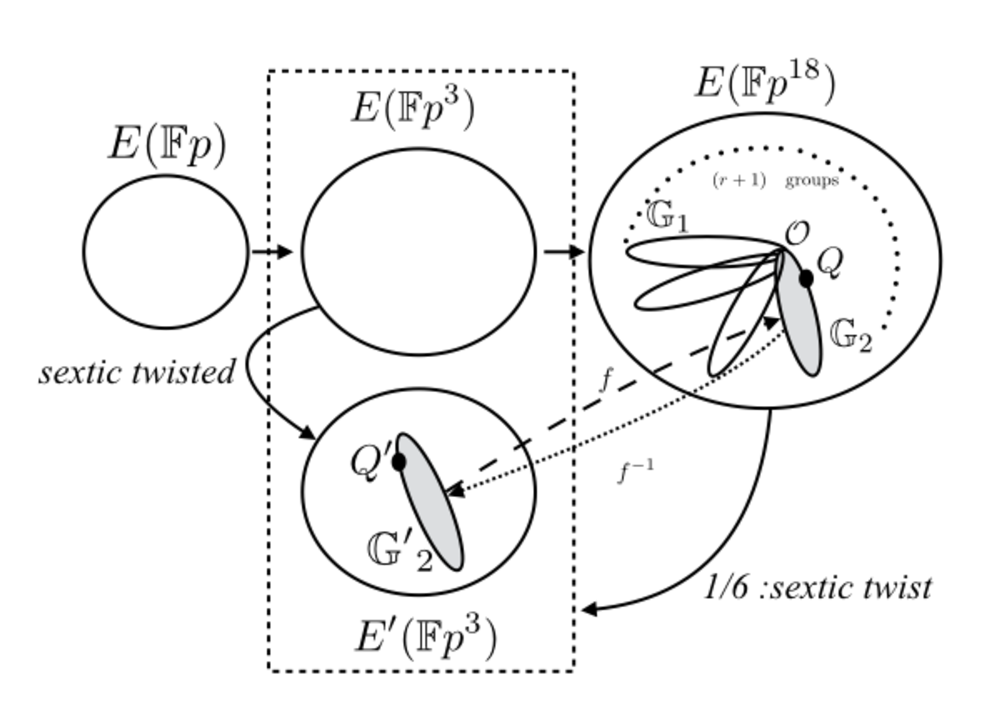
\includegraphics[width=3.5in]{twist.eps}
        \caption{\textit{sextic twist} in KSS curve.}
        \label{fig:sextic}
        \end{figure*}
        Let us consider $E$ is the KSS curve in base field $\FQTH$  and $E'$ is sextic twist of $E'$ given as follows: 
        \begin{eqnarray}
        E:y^2 & = &x^3+b,\\
        E':y^2 & = & x^3+bi, \label{eq:KSS_Twist}
        \end{eqnarray}
        where $b \in \Fp$; $x, y, i \in \FQTH$ and basis element $i$ is the quadratic and cubic non residue in $\FQTH$.
        
        In context of KSS curve, let us consider a rational point $Q\in \g2 \subset E(\F{p}{18})$.
        $Q$ has a  special vector representation with 18 $\Fp$ elements for each $x_Q$ and $y_Q$ coordinates.
        Figure \ref{fig:Q_structure} shows the structure of the coefficients of $Q \in \FQEN$ and its sextic twisted isomorphic rational point $Q' \in \FQTH$ in KSS curve.
        \begin{figure*}
        \centering
        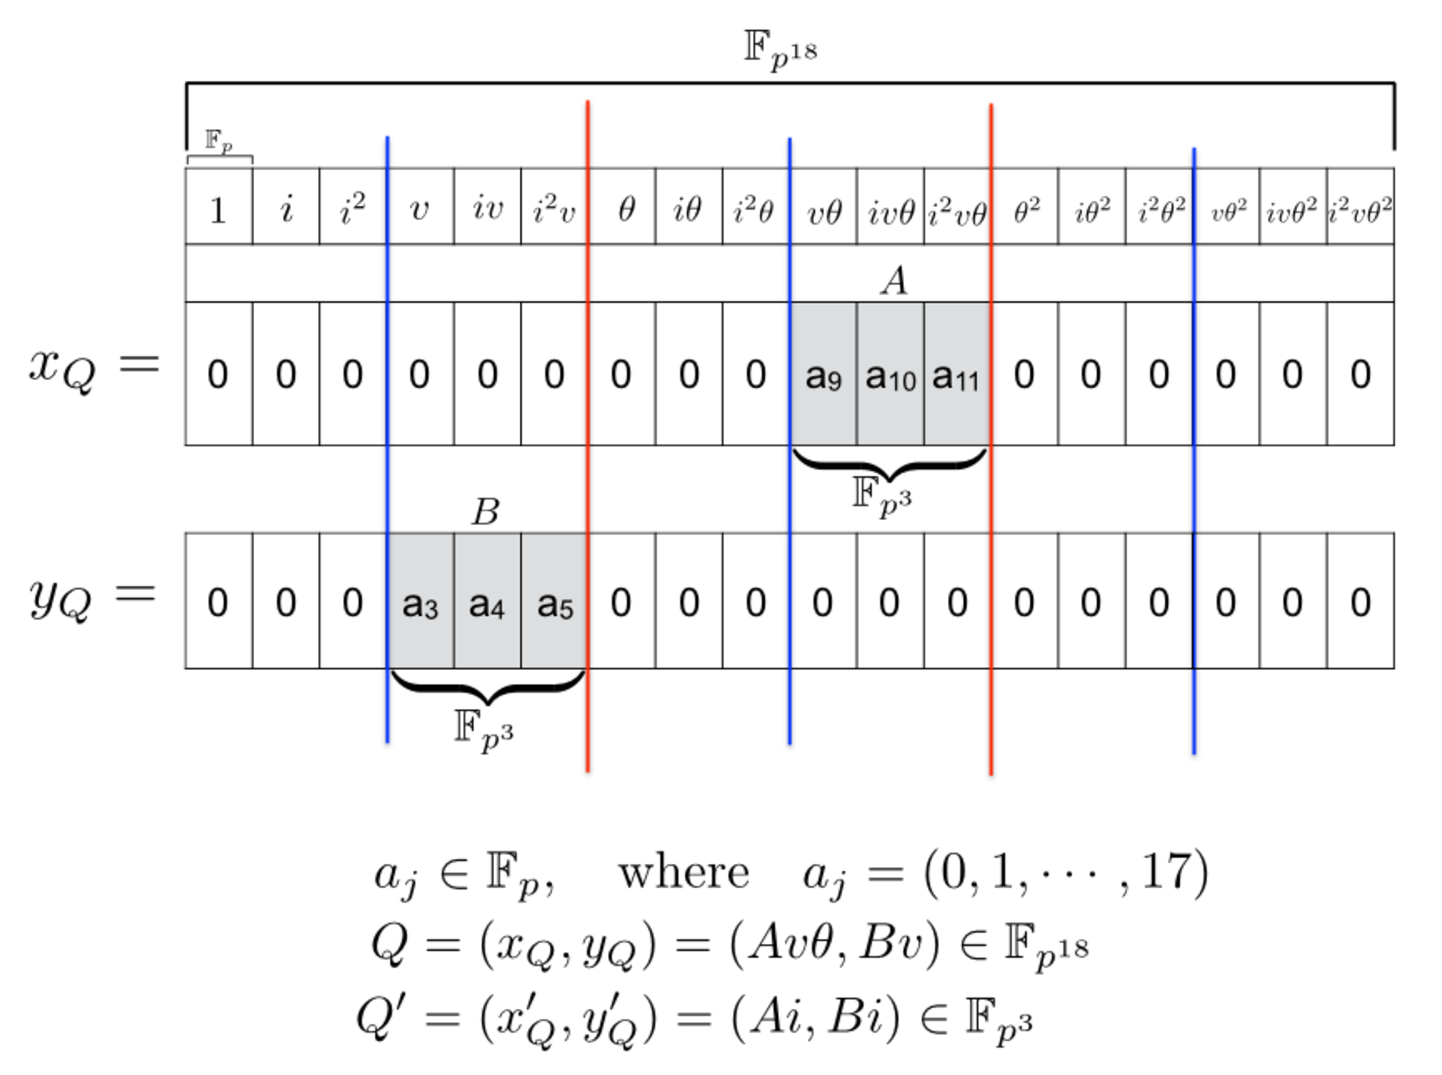
\includegraphics[width=4.5in]{structure.eps}
        \caption{ $Q \in \FQEN$ and its sextic twisted isomorphic rational point $Q' \in \FQTH$ structure in KSS curve.}
        \label{fig:Q_structure}
        \end{figure*}
        Among 18 elements, there are 3 continuous nonzero $\Fp$ elements. The others are zero.
        However the set of these nonzero elements belongs to $\FQTH$. 
        
        This thesis considers the mother parameter of KSS curve $u=65$-bit and characteristics $p=511$-bit. In such consideration, $Q$ is given as $Q = (Av\theta, Bv)$,  showed in Figure \ref{fig:Q_structure}, where $A, B \in \FQTH$ and $v$ and $\theta$ are the basis elements of $\F{p}{6}$ and $\FQEN$ respectively. 
        
        Let us consider the sextic twisted isomorphic subfield rational point of $Q$ as $Q' \in \g2' \subset E'(\F{p}{3})$.
        Considering $x'$ and $y'$ as the coordinates of $Q'$, we can map the rational point $Q = (Av\theta, Bv)$  to the rational point  $Q' = (x',y')$ as follows.
        
        Multiplying both side of \eqref{eq:KSS_Twist} with $\theta^{-6}$, where $i=\theta^6$ and $v = \theta^3$.
        \begin{equation}\label{eq.sextic_div_theta}
        E':  \Big(\frac{y}{\theta^3}\Big)^2  = \Big(\frac{x}{\theta^2}\Big)^3+ b.
        \end{equation}
         $\theta^{-2}$ of  \eqref{eq.sextic_div_theta} can be represented as follows:
         \begin{subequations}
         \begin{eqnarray}
         \theta^{-2} & = & i^{-1}i \theta^{-2}, \nonumber \\
         &  = & i^{-1}\theta^{4}, \label{thta2_4}
         \end{eqnarray}
         and multiplying $i$ with both sides.
         \begin{equation} \label{the4_2}
         \theta^4 = i\theta^{-2}.
         \end{equation}
        Similarly $\theta^{-3}$ can be represented as follows:
         \begin{eqnarray}
         \theta^{-3} & = & i^{-1}i \theta^{-3} \nonumber \\
         &   = & i^{-1}\theta^{3}.\label{thta_3} 
         \end{eqnarray}
         Multiplying $i$ with both sides of \eqref{thta_3} we get $\theta^3$ as,
         \begin{equation}\label{thta_3_3}
         \theta^3 = i\theta^{-3},
         \end{equation}
         \end{subequations}
        
        \subsubsection{$Q$ to $Q'$ mapping}
        Let us represent $Q = (Av\theta, Bv)$  as follows:
        \begin{equation}\label{18_to3}
        Q  =  (A\theta^4, B\theta^3), \quad \text{where $v=\theta^3$}.
        \end{equation}
        From \eqref{the4_2} and \eqref{thta_3_3}, we substitute $ \theta^4 = i\theta^{-2}$ and $\theta^3 = i\theta^{-3}$  in \eqref{18_to3}  as 
        follows:
        \begin{equation}\label{18_to3.1}
        Q  =  (Ai\theta^{-2}, Bi\theta^{-3}),
        \end{equation}
        where $Ai = x'$ and $Bi = y'$ are the coordinates of $Q' =(x',y') \in \FQTH$. Which implies that we can map $Q \in \FQEN$ to $Q' \in \FQTH$ by first selecting the $3$ nonzero $\Fp$ coefficients of each coordinates of $Q$. Then these nonzero $\Fp$ elements form an $\FQTH$ element. After that multiplying the basis element $i$ with that $\FQTH$ element, we get the final $Q' \in \FQTH$. From the structure of $\FQEN$, given in \eqref{eq:KSS_towering}, this mapping has required no expensive arithmetic operation.  Multiplication by the basis element $i$ in $\FQTH$ can be done by 1 bit wise left shifting since $c=2$ is considered for towering in \eqref{eq:KSS_towering}.
        
        \subsubsection{$Q'$ to $Q$ mapping}
         The reverse mapping $Q' =(x',y') \in \FQTH$ to $Q =(Av\theta,Bv) \in \FQEN$ can be obtained as from \eqref{thta2_4}, \eqref{thta_3} and \eqref{eq.sextic_div_theta} as follows:
         \begin{subequations}
         \begin{eqnarray}
         x i^{-1}\theta^{4} & = & Av\theta, \nonumber \\
         y i^{-1}\theta^{3} & = & Bv, \nonumber
         \end{eqnarray}
         \end{subequations}
          which resembles that $Q= (Av\theta, Bv)$. Therefore it means that multiplying $i^{-1}$ with the $Q'$ coordinates and placing the resulted coefficients in the corresponding position of the coefficients in $Q$, will map $Q'$ to $Q$.
        This mapping costs one $\FQTH$ inversion of $i$ which can be pre-computed and one $\Fp$ multiplication.
        
        
        \section{Result Analysis}
        In order to determine the advantage of the proposal, first we have applied the proposed mapping technique to map rational point $Q \in \g2 \subset E(\F{p}{18})$ to its isomorphic point $Q' \in \g2' \subset E'(\F{p}{3})$. After that we performed the scalar multiplication of $Q'$. Then the resulted points are re-mapped to $\g2$ in $\FQEN$. On the other hand we performed scalar multiplication of $Q$ without mapping. In the experiment, 100 scalar numbers of size (about 377-bit) less than order $r$ is generated randomly and then scalar multiplication is calculated for both case. Average value of execution time is considered for comparison.
        The comparative result is shown in Table \ref{tab_opeation}.
        
        In the experiment, mother parameter $u$ is also selected accordingly to find out $\g2$ rational point $Q$. In addition $p=511$-bit is considered, since Scott et al. \cite{IMA:Scott11} has proposed the size of the characteristics $p$ to be 508 to 511-bit with order $r$ of 384-bit for 192-bit security level.
        
        In the experiment, KSS curve over $\FQEN$ is given as $y^2 = x^3 + 11$, considering the following parameters
        \begin{eqnarray}
        u & = & 65   \mbox{-bit},  \nonumber \\ 
        p  & = & 511 \mbox{-bit},  \nonumber \\ 
        r  & = & 378 \mbox{-bit} ,\nonumber \\ 
        t  & = & 255  \mbox{-bit}. \nonumber
        \end{eqnarray}
        
        Table \ref{tab1} shows the experiment environment, used to evaluate usefulness of the proposed mapping.  
        \renewcommand{\baselinestretch}{1.5}
        \begin{table*}
        \renewcommand{\arraystretch}{1.3}
        \centering
        \caption{ Computational Environment}
        \label{tab1}
        \begin{tabular}{|c|c|c|}
        \hline 
        • & PC & iPhone6s \\ 
        \hline \hline 
        CPU {\textsuperscript{*}} & \quad 2.7 GHz Intel Core i5 \quad & \quad Apple A9 Dual-core 1.84 GHz \quad \\ 
        \hline 
        Memory & 16 GB & 2 GB \\ 
        \hline 
        OS & Mac OS X 10.11.4 &  iOS 9.3.1 \\ 
        \hline 
        Compiler & gcc 4.2.1 & gcc 4.2.1 \\ 
        \hline 
        \quad Programming Language \quad  & C & Objective-C, C \\ 
        \hline 
        Library & GNU MP \cite{gmp} & GNU MP \\ 
        \hline 
        \multicolumn{3}{l}{\textsuperscript{*}\footnotesize{Only single core is used from two cores.}}\\
        \end{tabular} 
        \end{table*}
        \renewcommand{\baselinestretch}{1.0}
        
        \renewcommand{\baselinestretch}{1.5}
        \begin{table*}
        %\renewcommand{\arraystretch}{1.3}
        \centering
        \caption{ Comparative result of average execution time in [ms] for scalar multiplication}
        \label{tab_opeation}
        \begin{tabular}{|c|c|c|c|}
        \hline
         & \multicolumn{3}{|c|}{\quad Average execution time [ms] comparison \quad} \\ \hline
        & PC & \multicolumn{2}{|c|}{iPhone 6s}  \\ 
         \hline \hline
         & \quad Execution time \quad & \multicolumn{2}{|c|}{\quad Execution time}\\ 
         \hline
        Binary method  with mapping &  $5.4 \times 10^1 $  &  \multicolumn{2}{|c|} { $6.4 \times 10^1$}\\ \hline
        Binary method  without mapping  &  $1.1 \times 10^3$  &  \multicolumn{2}{|c|} { $1.2 \times 10^3$}\\ \hline
        Montgomery ladder  with mapping &  $6.8 \times 10^1 $  &  \multicolumn{2}{|c|} { $8.4 \times 10^1$}\\ \hline
        Montgomery ladder  without mapping  &  $1.5 \times 10^3$  &  \multicolumn{2}{|c|} { $1.6 \times 10^3$}\\ \hline
        \end{tabular} 
        \end{table*}
        \renewcommand{\baselinestretch}{1.0}
        
        Analyzing  Table \ref{tab_opeation}, we can find that scalar multiplication using the proposed  mapping technique  is more than 20 times faster than scalar multiplication without the proposed mapping. It this experiment we used binary method and Montgomery ladder for scalar multiplication in both case. In the previous work of Nogami et al. \cite{DBLP:journals/ieicet/NogamiSONAM09}, has showed the procedure to apply Frobenious mapping on twisted elliptic curve for Ate-based pairing. This multiplication can be done more efficiently if skew Frobenius mapping is applied on sextic twisted isomorphic rational point after applying the proposed mapping. 
        
        In the experiment we have used two execution environments; such as PC and iPhone with different CPU frequencies. In both environments only one processor core is utilized. The result also shows that the ratio of execution time of PC and iPhone without mapping  of both methods is about 0.9. On the other hand the ratio of execution time with mapping  of both methods is about 0.8. But the ratio of CPU frequencies of  iPhone and PC is about $1.84 / 2.7 \approx 0.68$. Since PC and iPhone has different processor architectures therefore it's frequency ratio has no relation with the execution time ratio. 
        
        The main focus of this experiment is to evaluate the  acceleration ratio of scalar multiplication by applying the proposed mapping on $\g2$ rational point group of  KSS curve of embedding degree 18. The experiment does not focus on efficiently implementing scalar multiplication for certain environment. There are other pairing friendly curves such as BLS-12, BLS-24 \cite{EPRINT:FreScoTes06} where sextic twist is available. We will try to apply the proposed mapping on those curves as our future work.
        
        \section{Conclusion and future work}
        In this thesis we have proposed mapping procedure of $\g2$ rational point group to its sextic twisted subfield isomorphic rational point group $\g2'$  and its reverse mapping on KSS curve in context of Ate based pairing. 
        We have also presented the advantages of such mapping by applying binary scalar multiplication and Montgomery ladder on sextic twisted isomorphic rational points in $\g2'$. 
        Then result of  scalar multiplication in $\g2'$ can accelerate the scalar multiplication in $\g2 \subset E(\FQEN)$ by more than 20 times than scalar multiplication of $\g2$ rational point directly in $\FQEN$. In the previous work of Sakemi et al. \cite{CANS:SNOKM08} has proposed skew Frobenious map for $\g1$ rational point defined over BN curve. As a future work we would like to apply such approach on $\g1$ rational point defined over KSS curve. Together with the proposed mapping and the skew Frobenius mapping of $\g1$ will remarkably accelerate scalar multiplication over KSS curve in the context of pairing based cryptography.  
        
        %As a future work we would like to enhance the scalar multiplication in  subfield isomorphic rational point group by applying Frobenius mapping and some multi-scalar multiplication technique.  
        
        
        \section*{Acknowledgment}
        This work was partially supported by the Strategic Information and Communications R\&D Promotion Programme (SCOPE) of Ministry of Internal Affairs and Communications, Japan.
        
        
        